\documentclass[11pt]{article}
\usepackage[utf8]{inputenc}

% PACKAGES %%%%%%%%%%%%%%%%%%%%%%%%%%%%%%%%%%%%%%%%%%%%%%%%%%%%%%%%%%%%%%%%%%%%%

\usepackage{amsmath,amssymb}
\usepackage[T1]{fontenc} % font encoding
\usepackage{graphicx} % for figures
\usepackage{float} % for figures
\usepackage{indentfirst} % indent first paragraph of section
\usepackage{soul,xcolor} % for colors
\usepackage{xkcdcolors} % colors from XKCD color survey
\usepackage{mathtools} % for boxed equations within \align
\usepackage{sectsty} % adjust section headers
\usepackage{fancyhdr} % page headers
\usepackage{titling} % reference title,author,date (in fancyhdr page header)
\usepackage{breqn} % automatically line wrap long Eqs.
\usepackage{pdfpages} % for \includepdf
\usepackage{pdflscape} % landscape 
\usepackage{mdframed} % for framed environment
\usepackage{minted} % for syntax-highlighted code blocks
\usepackage{inconsolata} % better monospace font
\usepackage[letterpaper, total={6.5in, 9in}]{geometry} % set paper and margin size
\usepackage{empheq} % multiline boxed equations, etc.
\usepackage{hyperref} % hyperlinked references?
\usepackage{dsfont}	% gives you \mathds{} font
\usepackage{multirow} % merged cells in tabular
% \usepackage{enumerate} % custom enumerate numbering (or lettering in this case)
\usepackage[shortlabels]{enumitem} % more enumerate options
\usepackage{svg} % use inkscape to import svgs
\usepackage{bm} % bold symbols
\usepackage[parfill]{parskip} % replace indentation with paragraph spacing
\usepackage{nicematrix} % extended matrix features
\usepackage{nomencl} % nomenclature section
\usepackage{etoolbox} % nomenclature subsections among other things

% FORMATTING %%%%%%%%%%%%%%%%%%%%%%%%%%%%%%%%%%%%%%%%%%%%%%%%%%%%%%%%%%%%%%%%%%%

% add page headers
\pagestyle{fancy}
\fancyhf{}
\fancyhead[LE,LO]{\thetitle}
\fancyhead[RE,RO]{\theauthor}
\fancyfoot[CE,CO]{\thepage}

% adjust section header font size
\sectionfont{\fontsize{20}{15}\selectfont}
\subsectionfont{\fontsize{14}{15}\selectfont}


% LISTINGS %%%%%%%%%%%%%%%%%%%%%%%%%%%%%%%%%%%%%%%%%%%%%%%%%%%%%%%%%%%%%%%%%%%%%

% set code block formats
\definecolor{code_bg}{gray}{0.95}
\definecolor{console_bg}{gray}{1.00}
\setminted{
    bgcolor=code_bg,
    fontsize=\small,
    linenos,
    autogobble}
\setminted[python-console]{
    bgcolor=console_bg,
    linenos=false
    }

% NOMENCLATURE TABLE %%%%%%%%%%%%%%%%%%%%%%%%%%%%%%%%%%%%%%%%%%%%%%%%%%%%%%%%%%%
\renewcommand\nomgroup[1]{%
  \item[\bfseries
  \ifstrequal{#1}{A}{Acronyms}{%
  \ifstrequal{#1}{S}{Symbols}{%
  \ifstrequal{#1}{N}{Notation}{}}}%
]}

% MATH MACROS %%%%%%%%%%%%%%%%%%%%%%%%%%%%%%%%%%%%%%%%%%%%%%%%%%%%%%%%%%%%%%%%%%

% real and imaginary components
\renewcommand{\Re}{\operatorname{Re}}
\renewcommand{\Im}{\operatorname{Im}}

% Fourier transforms
% \newcommand\fourier[1]{\frac{1}{\sqrt{2\pi}} \int_{-\infty}^\infty #1 e^{-i\omega x} \textrm{d}x}
% \newcommand\inverseFourier[1]{\frac{1}{\sqrt{2\pi}} \int_{-\infty}^\infty #1 e^{i\omega x} \textrm{d}\omega}
\newcommand\fourier[1]{\int_{-\infty}^\infty #1 e^{-i\omega x} \textrm{d}x}
\newcommand\inverseFourier[1]{\frac{1}{2\pi} \int_{-\infty}^\infty #1 e^{i\omega x} \textrm{d}\omega}

% derivatives
\newcommand{\ppf}[2]{\frac{\partial #1}{\partial #2}}
\newcommand{\pppf}[3]{\frac{\partial^2 #1}{\partial #2 \partial #3}}
\newcommand{\ddf}[2]{\frac{\text{d} #1}{\text{d} #2}}
\newcommand{\DDf}[2]{\frac{\text{D} #1}{\text{D} #2}}

% norms
\newcommand\norm[1]{\left\lVert#1\right\rVert}

% statistical operators
\newcommand{\prob}{\operatorname{P}}
\newcommand{\expectation}{\operatorname{E}}
\newcommand{\variance}{\operatorname{Var}}
\newcommand{\stddev}{\operatorname{SD}}

% statistical distributions
\newcommand{\bernoulli}{\operatorname{Bernoulli}}
\newcommand{\binomial}{\operatorname{Binomial}}
\newcommand{\poisson}{\operatorname{Poisson}}
\newcommand{\normal}{\operatorname{Normal}}

% hyperbolic trig inverse functions
\DeclareMathOperator{\sech}{sech}
\DeclareMathOperator{\csch}{csch}
\DeclareMathOperator{\arcsec}{arcsec}
\DeclareMathOperator{\arccot}{arcCot}
\DeclareMathOperator{\arccsc}{arcCsc}
\DeclareMathOperator{\arccosh}{arcCosh}
\DeclareMathOperator{\arcsinh}{arcsinh}
\DeclareMathOperator{\arctanh}{arctanh}
\DeclareMathOperator{\arcsech}{arcsech}
\DeclareMathOperator{\arccsch}{arcCsch}
\DeclareMathOperator{\arccoth}{arcCoth} 

% highlighting in math mode
\newcommand{\mathhl}[1]{\colorbox{yellow}{$\displaystyle #1$}}

% COMMONLY USED COPYPASTAS %%%%%%%%%%%%%%%%%%%%%%%%%%%%%%%%%%%%%%%%%%%%%%%%%%%%%

%% CODE BLOCK

% \begin{listing}[H]
%     \caption{Code and output}
%     \label{lst1}
%     \begin{minted}{python}
%         import numpy as np
%         A = np.array([1, 2, 3])
%         print('Hello World')
%     \end{minted}
%     \begin{minted}{python-console}
%         Hello World
%     \end{minted}
% \end{listing}

% \inputminted{python}{helloworld.py}



%% MULTIPLE EQUATIONS BOXED

% \begin{empheq}[box=\fbox]{align}
% \end{empheq}



%% ENUMERTATE WITH a) instead of 1.

% \begin{enumerate}[label=\alph*)]
% \end{enumerate}



%% SET CURRENT SUBHEADER NUMBER

% \setcounter{subsection}{1}
% 'Problem' sections
\renewcommand{\thesection}{\arabic{section}}
\renewcommand{\thesubsection}{\arabic{section}.\alph{subsection}}
\renewcommand{\thesubsubsection}{\arabic{section}.\alph{subsection}.\roman{subsubsection}}
% \renewcommand{\thesubsection}{\arabic{subsection}}


\title{ENGR 520 Homework 3}
\author{Anthony Su}
\date{May 13, 2025}

\begin{document}
\thispagestyle{plain}
\maketitle

\textbf{Collaboration statement:} I did not collaborate with others on this assignment. I utilized large
language models for code debugging.

%%%%%%%%%%%%%%%%%%%%%%%%%%%%%%%%%%%%%%%%%%%%%%%%%%%%%%%%%%%%%%%%%%%%%%%%%%%%%%%%
% 1. 
%%%%%%%%%%%%%%%%%%%%%%%%%%%%%%%%%%%%%%%%%%%%%%%%%%%%%%%%%%%%%%%%%%%%%%%%%%%%%%%%
\section{}

This section discusses modeling the Lotka-Volterra (L-V) Predator-Prey system using sparse identification of nonlinear dynamics (SINDy). The L-V system is defined as:
\begin{align*}
    \dot{x}_1 &= \alpha x_1 - \beta x_1 x_2 \\
    \dot{x}_2 &= \delta x_1 x_2 - \gamma x_2
\end{align*}
A SINDy model is found by solving the following linear system:
\begin{equation*}
    \dot{\mathbf{X}} = \mathbf{\Theta}(\mathbf{X}) \mathbf{\Xi}
\end{equation*}
where $\mathbf{X}$ are the data, $\mathbf{\Theta}$ are the library of candidate functions, and $\mathbf{\Xi}$ are the coefficients of $\mathbf{\Theta}$. In this report, $\mathbf{\Theta}$ are polynomial functions and the solution is found via sequentially-thresholded least-squares (STLS).


\subsection{} % a --------------------------------------------------------------

Figure \ref{p1afig1} shows the phase portrait of this model as it is simulated on the interval $t=[0, 10]$.

\begin{figure}[H]
    \centering
    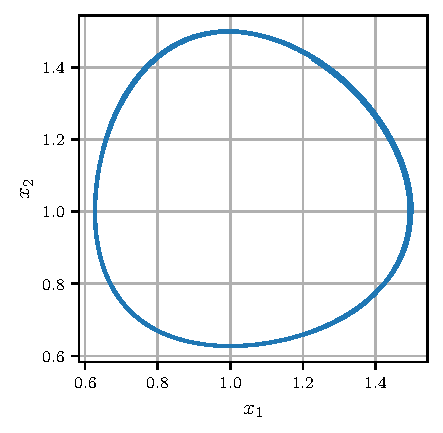
\includegraphics[width=3in]{p1fig1.pdf}
    \caption{Lotka-Volterra Model Phase Portrait}
    \label{p1afig1}
\end{figure}


\subsection{} % b --------------------------------------------------------------

Table \ref{p1btab1} shows the results of SINDy when using a 2nd-order polynomial library for $\mathbf{\Theta}$.

\begin{table}[H]
    \centering
    \caption{SINDy using STLS optimizer and 2nd-order polynomial library}
    \label{p1btab1}
    \begin{tabular}{|c|l|}
        \hline
        Threshold & Model \\
        \hline
        \hline
        \multirow{2}{*}{0.20} & $\dot{x}_1 = 2.001 x_1 - 2.001 x_1 x_2$ \\
                              & $\dot{x}_2 = -2.002 x_2 + 2.002 x_1 x_2$ \\
        \hline
        \multirow{2}{*}{0.19} & $\dot{x}_1 = 2.001 x_1 - 2.001 x_1 x_2$ \\
                              & $\dot{x}_2 = -2.002 x_2 + 2.002 x_1 x_2$ \\
        \hline
        \multirow{2}{*}{0.18} & $\dot{x}_1 = 2.001 x_1 - 2.001 x_1 x_2$ \\
                              & $\dot{x}_2 = -2.002 x_2 + 2.002 x_1 x_2$ \\
        \hline
        \multirow{2}{*}{0.17} & $\dot{x}_1 = 2.001 x_1 - 2.001 x_1 x_2$ \\
                              & $\dot{x}_2 = -2.002 x_2 + 2.002 x_1 x_2$ \\
        \hline
        \multirow{2}{*}{0.16} & $\dot{x}_1 = 2.001 x_1 - 2.001 x_1 x_2$ \\
                              & $\dot{x}_2 = 0.408 - 0.408 x_1 - 2.450 x_2 + 0.197 x_1^2 + 1.998 x_1 x_2 + 0.216 x_2^2$ \\
        \hline
        \multirow{2}{*}{0.15} & $\dot{x}_1 = -0.381 + 2.374 x_1 + 0.427 x_2 - 0.182 x_1^2 - 1.996 x_1 x_2 - 0.206 x_2^2$ \\
                              & $\dot{x}_2 = 0.408 - 0.408 x_1 - 2.450 x_2 + 0.197 x_1^2 + 1.998 x_1 x_2 + 0.216 x_2^2$ \\
        \hline
    \end{tabular}
\end{table}


\subsection{} % c --------------------------------------------------------------

For thresholds above 0.16, the discovered $\Xi$ matches well with the ground truth. For this system's sparse dynamics, a higher threshold performs well. For lower thresholds, some extra terms erroneously are included. As the threshold is modulated, the model's sparsity pattern changes in discrete and sudden jumps.


\subsection{} % d --------------------------------------------------------------

Table \ref{p1dtab1} shows the SINDy models of the L-V system when using a 3rd-order polynomial library for $\mathbf{\Theta}$.

\begin{table}[H]
    \centering
    \caption{SINDy L-V Models}
    \label{p1dtab1}
    \begin{tabular}{|c|l|}
        \hline
        Threshold & Model \\
        \hline
        \hline
        \multirow{2}{*}{0.20} & $\dot{x}_1 = 2.001 x_1 - 2.001 x_1 x_2$ \\
                              & $\dot{x}_2 = -2.002 x_2 + 2.002 x_1 x_2$ \\
        \hline
        \multirow{2}{*}{0.19} & $\dot{x}_1 = 2.001 x_1 - 2.001 x_1 x_2$ \\
                              & $\dot{x}_2 = -2.002 x_2 + 2.002 x_1 x_2$ \\
        \hline
        \multirow{2}{*}{0.18} & $\dot{x}_1 = 2.001 x_1 - 2.001 x_1 x_2$ \\
                              & $\dot{x}_2 = -2.002 x_2 + 2.002 x_1 x_2$ \\
        \hline
        \multirow{2}{*}{0.17} & $\dot{x}_1 = 2.001 x_1 - 2.001 x_1 x_2$ \\
                              & $\dot{x}_2 = -2.002 x_2 + 2.002 x_1 x_2$ \\
        \hline
        \multirow{2}{*}{0.16} & $\dot{x}_1 = 2.001 x_1 - 2.001 x_1 x_2$ \\
                              & $\dot{x}_2 = 0.408 - 0.408 x_1 - 2.450 x_2 + 0.197 x_1^2 + 1.998 x_1 x_2 + 0.216 x_2^2$ \\
        \hline
        \multirow{2}{*}{0.15} & $\dot{x}_1 = -0.381 + 2.374 x_1 + 0.427 x_2 - 0.182 x_1^2 - 1.996 x_1 x_2 - 0.206 x_2^2$ \\
                              & $\dot{x}_2 = 0.408 - 0.408 x_1 - 2.450 x_2 + 0.197 x_1^2 + 1.998 x_1 x_2 + 0.216 x_2^2$ \\
        \hline
    \end{tabular}
\end{table}

The results exactly match those from the 2nd-order polynomial solution. Thus, it was able to converge to the correct solution at higher thresholds. This implies that the system has no significant cubic-like behavior for the SINDy model to fit to.


\subsection{} % e --------------------------------------------------------------

Figure \ref{p1efig1} shows the trajectory of this model as it is simulated on the interval $t=[0, 10]$ with a small amount of noise added.

\begin{figure}[H]
    \centering
    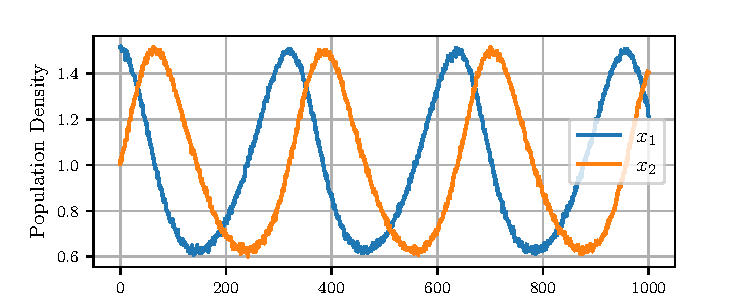
\includegraphics[width=5in]{p1fig2.pdf}
    \caption{Trajectory with $\sigma=0.01$ noise}
    \label{p1efig1}
\end{figure}

Table \ref{p1etab1} shows the SINDy models of the L-V system from noisy data when using a 3rd-order polynomial library for $\mathbf{\Theta}$.

\begin{table}[H]
    \centering
    \caption{SINDy L-V Models from noisy data}
    \label{p1etab1}
    \begin{tabular}{|c|l|}
        \hline
        Threshold & Model \\
        \hline
        \hline
        \multirow{2}{*}{0.20} & $\dot{x}_1 = 1.996 x_1 - 2.003 x_1 x_2$ \\
                            & $\dot{x}_2 = -2.013 x_2 + 2.015 x_1 x_2$ \\
        \hline
        \multirow{2}{*}{0.19} & $\dot{x}_1 = 1.996 x_1 - 2.003 x_1 x_2$ \\
                            & $\dot{x}_2 = -2.013 x_2 + 2.015 x_1 x_2$ \\
        \hline
        \multirow{2}{*}{0.18} & $\dot{x}_1 = 0.106 + 1.939 x_1 - 0.136 x_2 - 0.001 x_1^2 - 1.959 x_1 x_2 + 0.044 x_2^2$ \\
                            & $\dot{x}_2 = -2.013 x_2 + 2.015 x_1 x_2$ \\
        \hline
        \multirow{2}{*}{0.17} & $\dot{x}_1 = 0.106 + 1.939 x_1 - 0.136 x_2 - 0.001 x_1^2 - 1.959 x_1 x_2 + 0.044 x_2^2$ \\
                            & $\dot{x}_2 = -2.013 x_2 + 2.015 x_1 x_2$ \\
        \hline
        \multirow{2}{*}{0.16} & $\dot{x}_1 = 0.106 + 1.939 x_1 - 0.136 x_2 - 0.001 x_1^2 - 1.959 x_1 x_2 + 0.044 x_2^2$ \\
                            & $\dot{x}_2 = -2.013 x_2 + 2.015 x_1 x_2$ \\
        \hline
        \multirow{2}{*}{0.15} & $\dot{x}_1 = 0.106 + 1.939 x_1 - 0.136 x_2 - 0.001 x_1^2 - 1.959 x_1 x_2 + 0.044 x_2^2$ \\
                            & $\dot{x}_2 = -2.013 x_2 + 2.015 x_1 x_2$ \\
        \hline
    \end{tabular}
\end{table}

The noise increased the threshold required to obtain the correct model. It seems that SINDy is prone to overfitting in the presence of noise.



%%%%%%%%%%%%%%%%%%%%%%%%%%%%%%%%%%%%%%%%%%%%%%%%%%%%%%%%%%%%%%%%%%%%%%%%%%%%%%%%
% 2. 
%%%%%%%%%%%%%%%%%%%%%%%%%%%%%%%%%%%%%%%%%%%%%%%%%%%%%%%%%%%%%%%%%%%%%%%%%%%%%%%%
\section{}

This section discusses modeling the Lorenz system using SINDy.  The Lorenz system is defined as:
\begin{align*}
    \dot{x} &= \sigma (y - x) \\
    \dot{y} &= x (\rho - z) - y \\
    \dot{z} &= x y - \beta z
\end{align*}
where $\sigma=10$, $\rho=28$, and $\beta=8/3$.


\subsection{} % a --------------------------------------------------------------

Table \ref{p2atab1} shows the SINDy models of the Lorenz system when using a 2nd-order polynomial library for $\mathbf{\Theta}$ and a SLTS threshold of 0.2.

\begin{table}[H]
    \centering
    \caption{SINDy Lorenz models}
    \label{p2atab1}
    \begin{tabular}{|c|l|}
        \hline
        $t_{\text{end}}$ & Model \\
        \hline
        \hline
        \multirow{2}{*}{0.5} & $\dot{x} = -10.003 x + 10.003 y$ \\
                            & $\dot{y} = 0.247 1 + 28.081 x + -1.021 y + -1.000 x z$ \\
                            & $\dot{z} = -55.597 1 + 36.681 x + -20.192 y + 0.462 z + -1.891 x^2 + 1.803 x y + -1.312 x z + 0.498 y z$ \\
        \hline
        \multirow{2}{*}{1.0} & $\dot{x} = -9.992 x + 9.998 y$ \\
                            & $\dot{y} = 0.252 1 + 28.289 x + -1.095 y + -1.005 x z$ \\
                            & $\dot{z} = -2.662 z + 0.999 x y$ \\
        \hline
        \multirow{2}{*}{1.5} & $\dot{x} = -10.006 x + 10.007 y$ \\
                            & $\dot{y} = 9.241 1 + 3.013 x + 11.052 y + -0.732 z + 1.443 x^2 + -0.684 x y + -0.346 y z$ \\
                            & $\dot{z} = -2.665 z + 1.000 x y$ \\
        \hline
        \multirow{2}{*}{2.0} & $\dot{x} = -10.005 x + 10.005 y$ \\
                            & $\dot{y} = 27.782 x + -0.960 y + -0.992 x z$ \\
                            & $\dot{z} = -2.665 z + 0.999 x y$ \\
        \hline
    \end{tabular}
\end{table}


\subsection{} % b --------------------------------------------------------------

Data equivalent to that in Table \ref{p2atab1} was generated for several data sampling rates. These models were compared to the true equations of motion. Table \ref{p2btab1} shows which models had the same polynomial terms as the true equations. In other words, Table \ref{p2btab1} shows which models have the same sparsity matrix as the true model.

\begin{table}[H]
    \centering
    \caption{Sampling rates where SINDy recovers the true sparsity matrix}
    \label{p2btab1}
    \begin{tabular}{|c|c|c|c|c|c|}
        \cline{3-6}
        \multicolumn{2}{c|}{\multirow{2}{*}{}} & \multicolumn{4}{c|}{$\Delta t$} \\
        \cline{3-6}
        \multicolumn{2}{c|}{} & 0.0001 & 0.001 & 0.01 & 0.1 \\
        \hline
        \multirow{5}{*}{$t_{\text{end}}$} & 0.5 &  &  &  &  \\
        & 0.5 &  &  &  &  \\
        & 1.0 &  &  &  &  \\
        & 2.0 & \checkmark & \checkmark &  &  \\
        & 4.0 & \checkmark & \checkmark & \checkmark &  \\
        & 9.0 & \checkmark & \checkmark & \checkmark &  \\
        \hline
    \end{tabular}
\end{table}

Reducing sampling rate reduces the accuracy of the SINDy model.


\subsection{} % c --------------------------------------------------------------

Data equivalent to that in Table \ref{p2atab1} was generated for many magnitudes of noise added to the training data. These models were compared to the true equations of motion. Figure \ref{p2cfig1} shows the probability that models have the same sparsity matrix as the true model subject to various magnitudes of noise in the training data.

Note that the sampling rate in this study is the original $\Delta t = 0.0001$.

% \begin{table}[H]
%     \centering
%     \caption{Probability that SINDy recovers the true sparsity matrix at various noise magnitudes}
%     \label{p3btab1}
%     \begin{tabular}{|c|c|c|c|c|c|c|}
%         \cline{3-7}
%         \multicolumn{2}{c|}{\multirow{2}{*}{}} & \multicolumn{5}{c|}{noise $\sigma$} \\
%         \cline{3-7}
%         \multicolumn{2}{c|}{} & 0.00 & 0.01 & 0.05 & 0.10 & 0.50 \\
%         \hline
%         \multirow{6}{*}{$t_{\text{end}}$}
%         & 0.5 & 0.00 & 0.00 & 0.00 & 0.00 & 0.00 \\
%         & 1.0 & 0.18 & 0.00 & 0.00 & 0.00 & 0.00 \\
%         & 2.0 & 0.90 & 0.20 & 0.12 & 0.00 & 0.00 \\
%         & 4.0 & 1.00 & 0.86 & 0.46 & 0.00 & 0.00 \\
%         & 9.0 & 1.00 & 1.00 & 0.90 & 0.00 & 0.00 \\
%         \hline
%     \end{tabular}
% \end{table}

\begin{figure}[H]
    \centering
    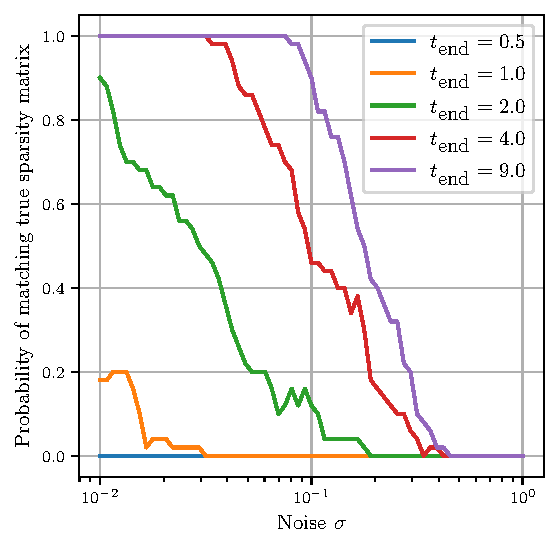
\includegraphics[width=4in]{p2fig2.pdf}
    \caption{SINDy performance vs. noise magnitude of various dataset lengths}
    \label{p2cfig1}
\end{figure}

Increasing the data noise reduces the accuracy of the SINDy model.



%%%%%%%%%%%%%%%%%%%%%%%%%%%%%%%%%%%%%%%%%%%%%%%%%%%%%%%%%%%%%%%%%%%%%%%%%%%%%%%%
% 3. 
%%%%%%%%%%%%%%%%%%%%%%%%%%%%%%%%%%%%%%%%%%%%%%%%%%%%%%%%%%%%%%%%%%%%%%%%%%%%%%%%
\section{}


\stepcounter{subsection}
\subsection{} % b --------------------------------------------------------------

Functions for forward difference numerical differentiation and central difference numerical differentiation are shown in Listings \ref{p3blst1} and \ref{p3blst2}.

\begin{listing}[H]
    \caption{Forward difference function}
    \label{p3blst1}
    \begin{minted}{python}
        def forward_difference(x: ArrayLike, t: ArrayLike=np.arange(len(x))) -> NDArray:
            """Forward difference numerical differentiation

            Args:
                x (ArrayLike): independent variable
                t (ArrayLike, optional): dependent variable. Defaults to np.arange(len(x)).

            Returns:
                NDArray: derivative of independent variable
            """
            dxdt = np.empty_like(x)
            dxdt[:-1] = (x[1:] - x[:-1]) / (t[1:] - t[:-1]).reshape(-1, 1)
            dxdt[-1] = dxdt[-2]
            return dxdt
    \end{minted}
\end{listing}

\begin{listing}[H]
    \caption{Central difference function}
    \label{p3blst2}
    \begin{minted}{python}
        def central_difference(x: ArrayLike, t: ArrayLike=np.arange(len(x))) -> NDArray:
            """Central difference numerical differentiation

            Args:
                x (ArrayLike): independent variable
                t (ArrayLike, optional): dependent variable. Defaults to np.arange(len(x)).

            Returns:
                NDArray: derivative of independent variable
            """
            dxdt = np.empty_like(x)
            dxdt[1:-1] = (x[2:] - x[:-2]) / (t[2:] - t[:-2]).reshape(-1, 1)
            dxdt[0] = dxdt[1]
            dxdt[-1] = dxdt[-2]
            return dxdt
    \end{minted}
\end{listing}


\subsection{} % c --------------------------------------------------------------

\begin{table}[H]
    \centering
    \caption{SINDy models using various differentiation schemes}
    \label{p3ctab1}
    \begin{tabular}{|c|l|}
        \hline
        $t_{\text{end}}$ & Model \\
        \hline
        \hline
        \multirow{2}{*}{Forward difference} & $\dot{x} = -9.992 x + 9.998 y$ \\
                            & $\dot{y} = 0.252 1 + 28.289 x + -1.095 y + -1.005 x z$ \\
                            & $\dot{z} = -2.662 z + 0.999 x y$ \\
        \hline
        \multirow{2}{*}{Central difference} & $\dot{x} = -9.985 x + 9.985 y$ \\
                            & $\dot{y} = 27.592 x + -0.916 y + -0.987 x z$ \\
                            & $\dot{z} = -2.660 z + 0.997 x y$ \\
        \hline
        \multirow{2}{*}{Smooth Difference} & $\dot{x} = -9.971 x + 9.971 y$ \\
                            & $\dot{y} = 27.420 x + -0.878 y + -0.983 x z$ \\
                            & $\dot{z} = -2.655 z + 0.995 x y$ \\
        \hline
    \end{tabular}
\end{table}

Using central difference and smooth difference schemes, SINDy  is able to converge to the correct model from the data. However, the model constants/coefficients are not as precise due to the noise.

\subsection{} % d --------------------------------------------------------------

For each of 65 noise magnitudes between 0.01 and 1, I generated 50 instantiations of noisy data. I fitted a SINDy model to each noisy dataset. The success rate of these models in matching the sparsity matrix of the true system are shown in Figure \ref{p3cfig1}.

\begin{figure}[H]
    \centering
    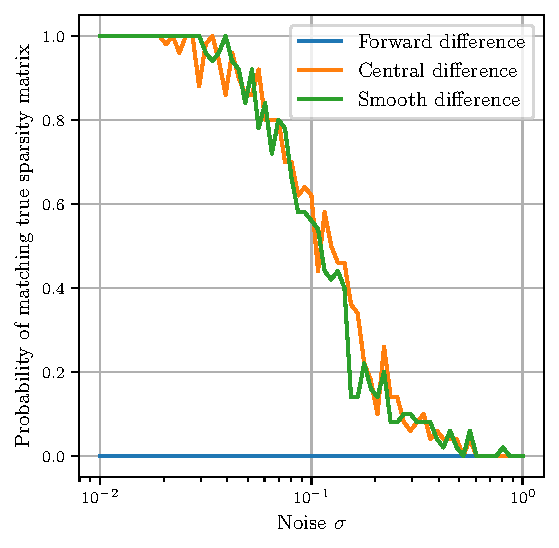
\includegraphics[width=4in]{p3fig1.pdf}
    \caption{SINDy performance vs. noise magnitude of various differentiation schemes}
    \label{p3cfig1}
\end{figure}

Using smooth difference and central difference schemes, SINDy is able to converge to the correct model if the noise is small. However, it is never able to do so using the forward difference scheme.



%%%%%%%%%%%%%%%%%%%%%%%%%%%%%%%%%%%%%%%%%%%%%%%%%%%%%%%%%%%%%%%%%%%%%%%%%%%%%%%%
% 4. 
%%%%%%%%%%%%%%%%%%%%%%%%%%%%%%%%%%%%%%%%%%%%%%%%%%%%%%%%%%%%%%%%%%%%%%%%%%%%%%%%
\section{}


\subsection{} % a --------------------------------------------------------------

The sparsest discovered SINDy model which supports the data is:
\begin{equation}
    u_t = -0.985 u_x - 0.010 u_{xxx} + -0.089 u u_{x}
\end{equation}
This model's solution is visualized in Figure \ref{p4afig1}.
\begin{figure}[H]
    \centering
    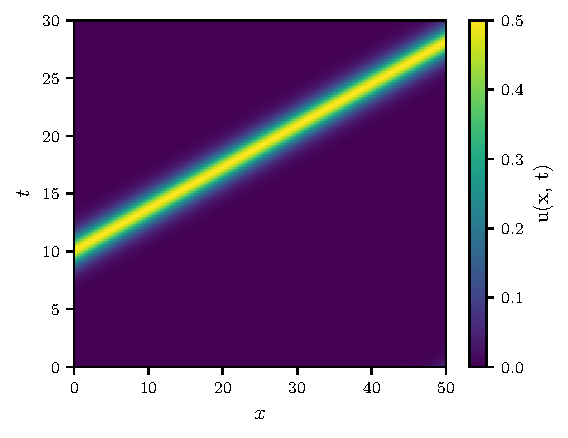
\includegraphics[width=4in]{p4fig1.pdf}
    \caption{SINDy model of Kortweg-De Vries system ($c=1$)}
    \label{p4afig1}
\end{figure}

This is the incorrect sparsity matrix for this system.

\subsection{} % b --------------------------------------------------------------

The sparsest discovered SINDy model which supports the concatenated data is:
\begin{equation*}
    u_t = -1.183 u_{xxx} + -6.192 u u_{x}
\end{equation*}
This model's solution is visualized in Figure \ref{p4bfig1}.
\begin{figure}[H]
    \centering
    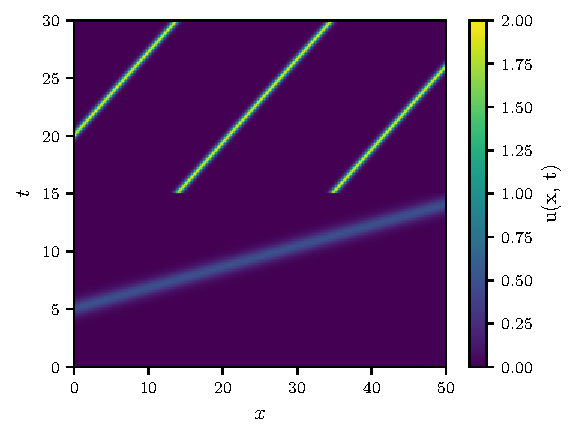
\includegraphics[width=4in]{p4fig2.pdf}
    \caption{SINDy model of Kortweg-De Vries system from concatenated data}
    \label{p4bfig1}
\end{figure}

This is the correct sparsity matrix for this system.


\subsection{} % c --------------------------------------------------------------
When training using only the first dataset, some features of the system were not expressed in the data. Thus, the sparse optimizer converged to a simpler system which was capable of matching the data.

In contrast, more features of the dataset and the underlying system were expressed in the concatenated dataset. Thus, the sparse optimizer converged to a more complex system which was capable of matching the data.


%%%%%%%%%%%%%%%%%%%%%%%%%%%%%%%%%%%%%%%%%%%%%%%%%%%%%%%%%%%%%%%%%%%%%%%%%%%%%%%%
% CODE APPENDIX
%%%%%%%%%%%%%%%%%%%%%%%%%%%%%%%%%%%%%%%%%%%%%%%%%%%%%%%%%%%%%%%%%%%%%%%%%%%%%%%%
\section*{Code Apendix}


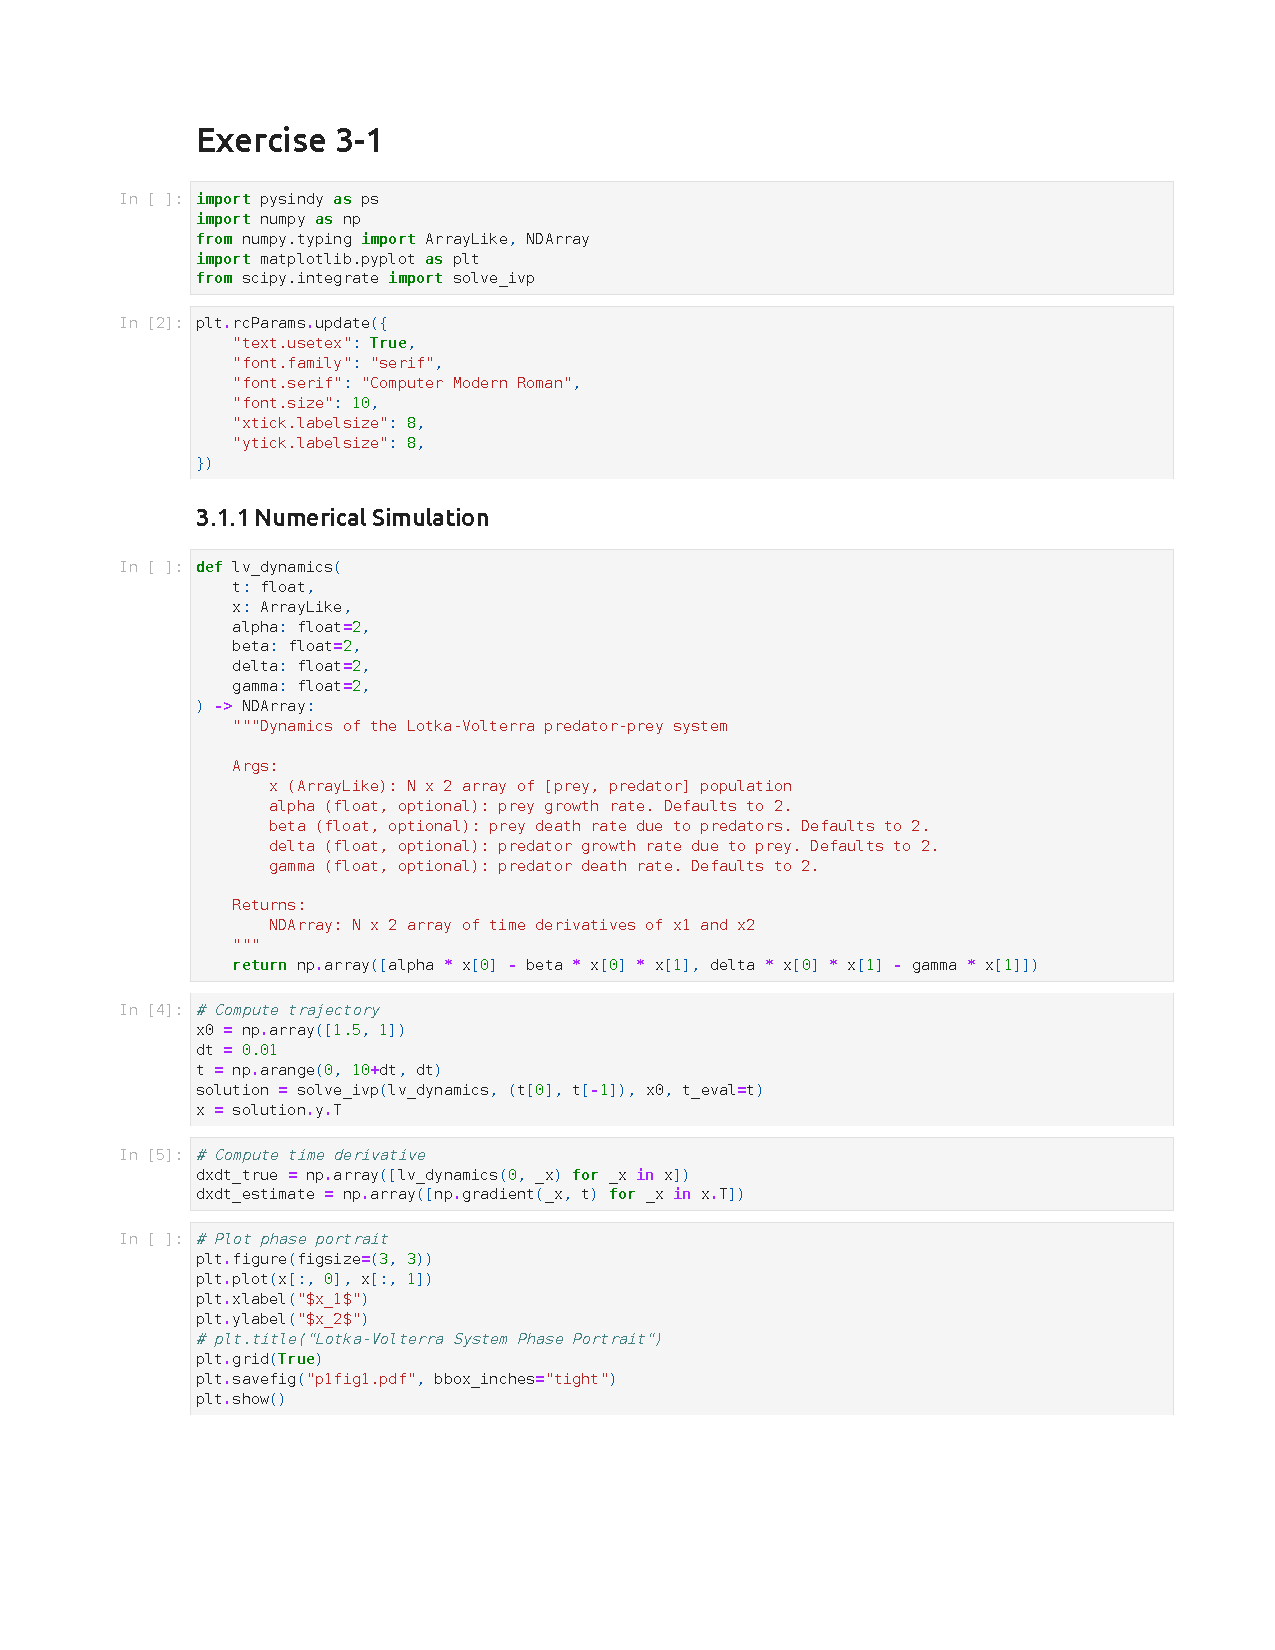
\includepdf[pages=-]{hw3p1.pdf}
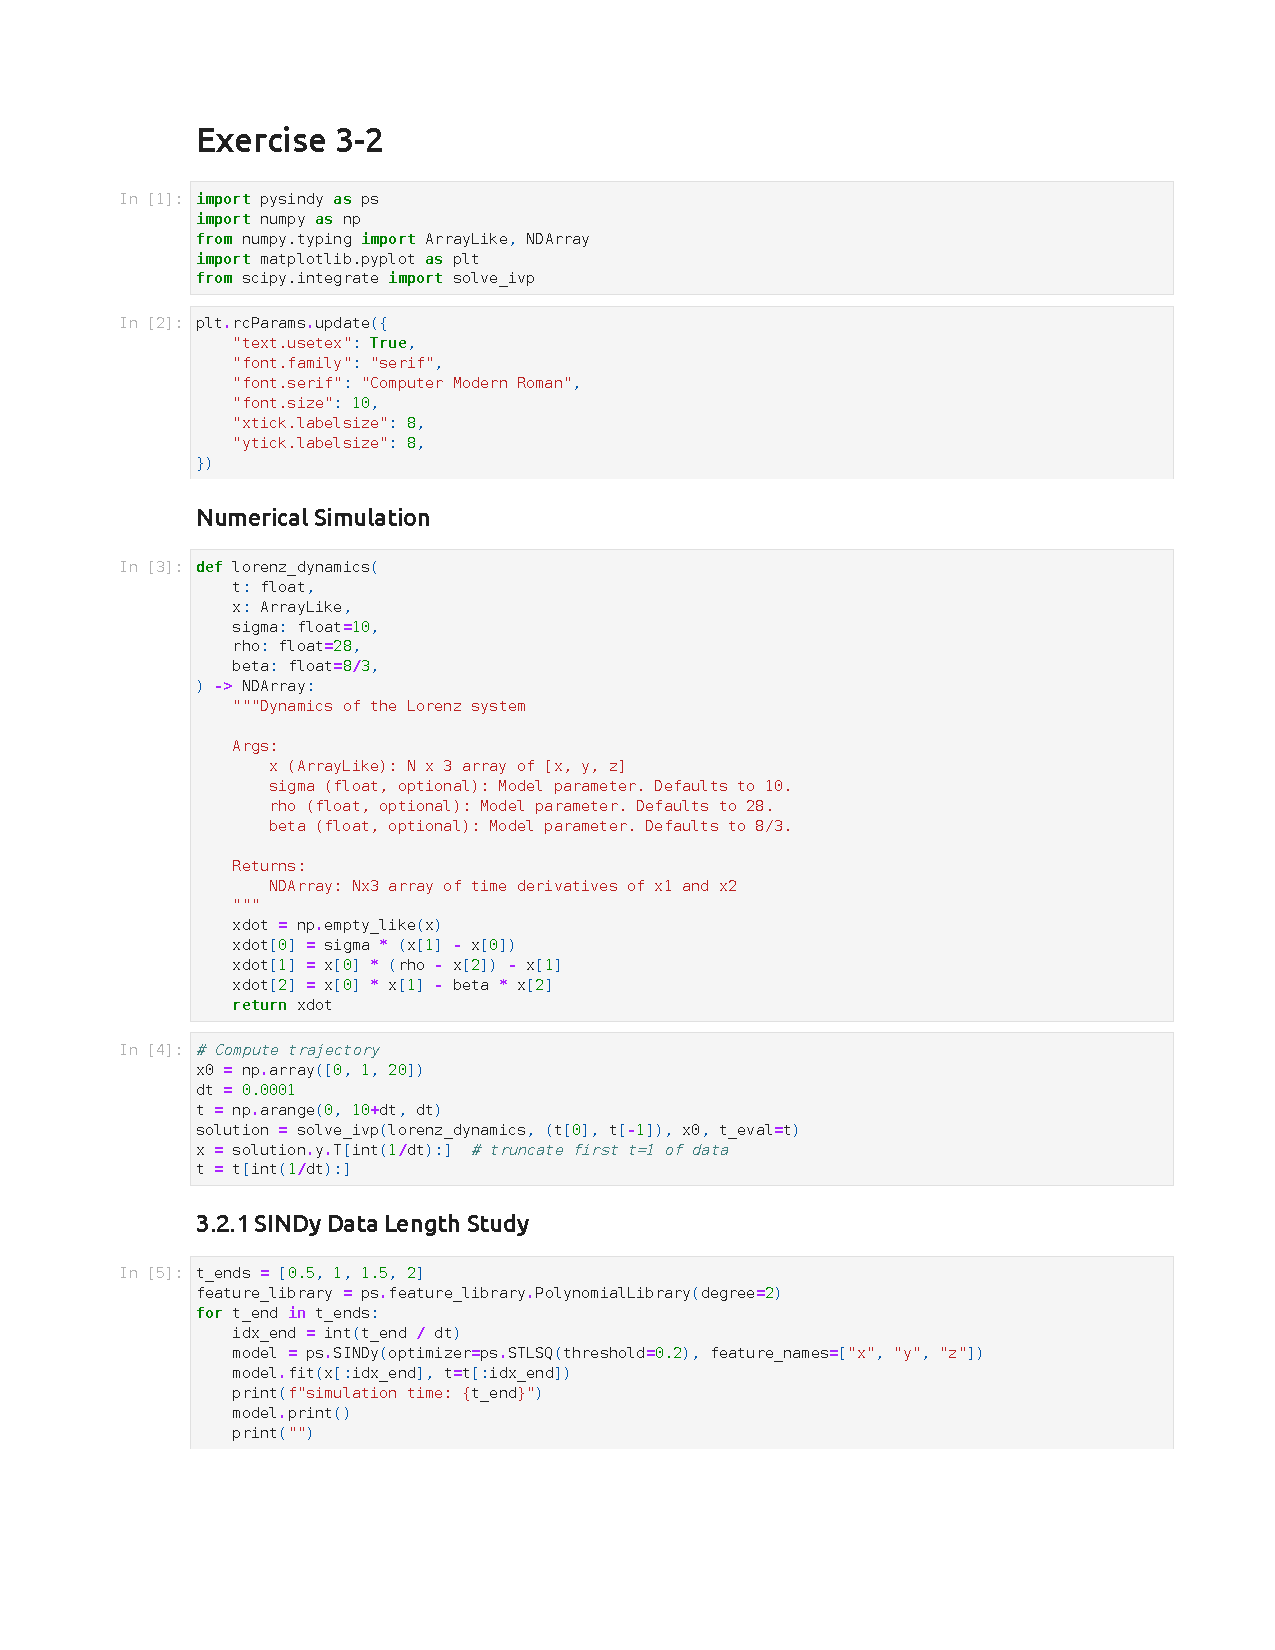
\includepdf[pages=-]{hw3p2.pdf}
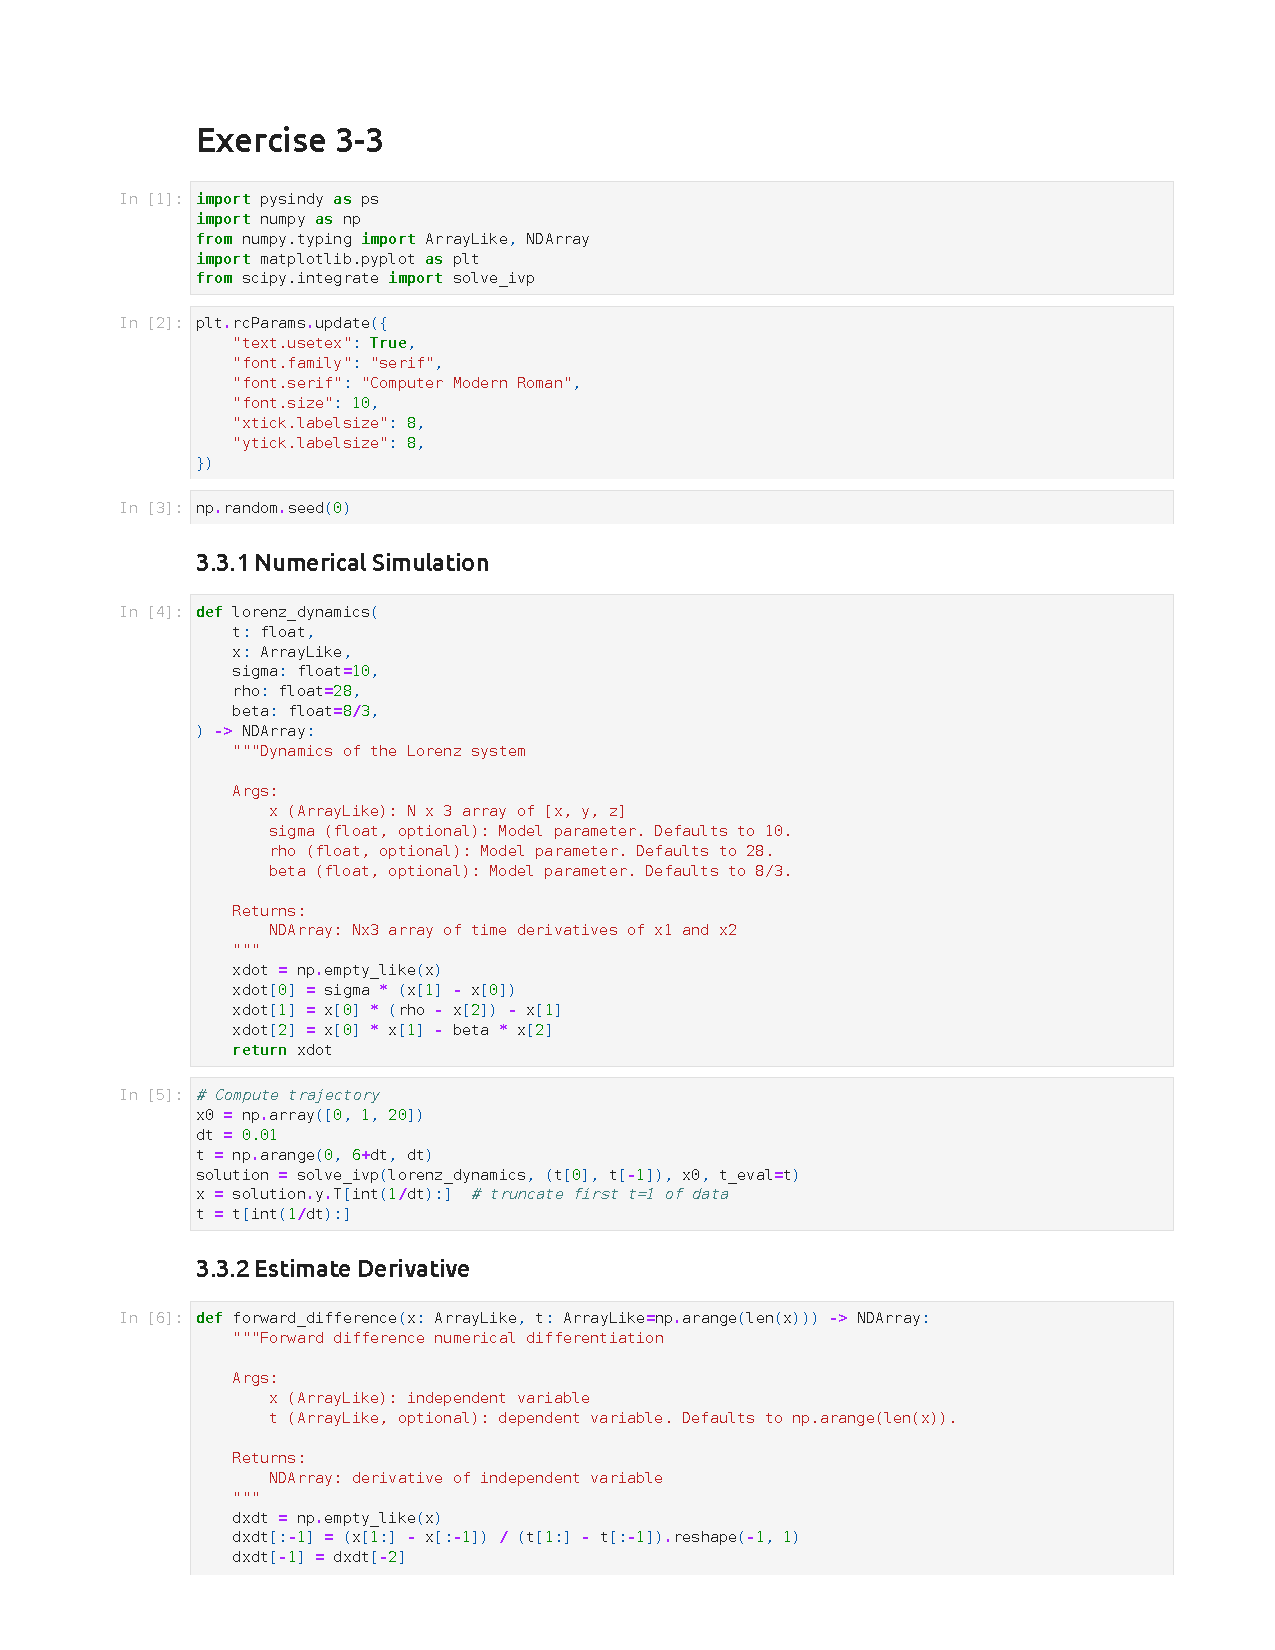
\includepdf[pages=-]{hw3p3.pdf}
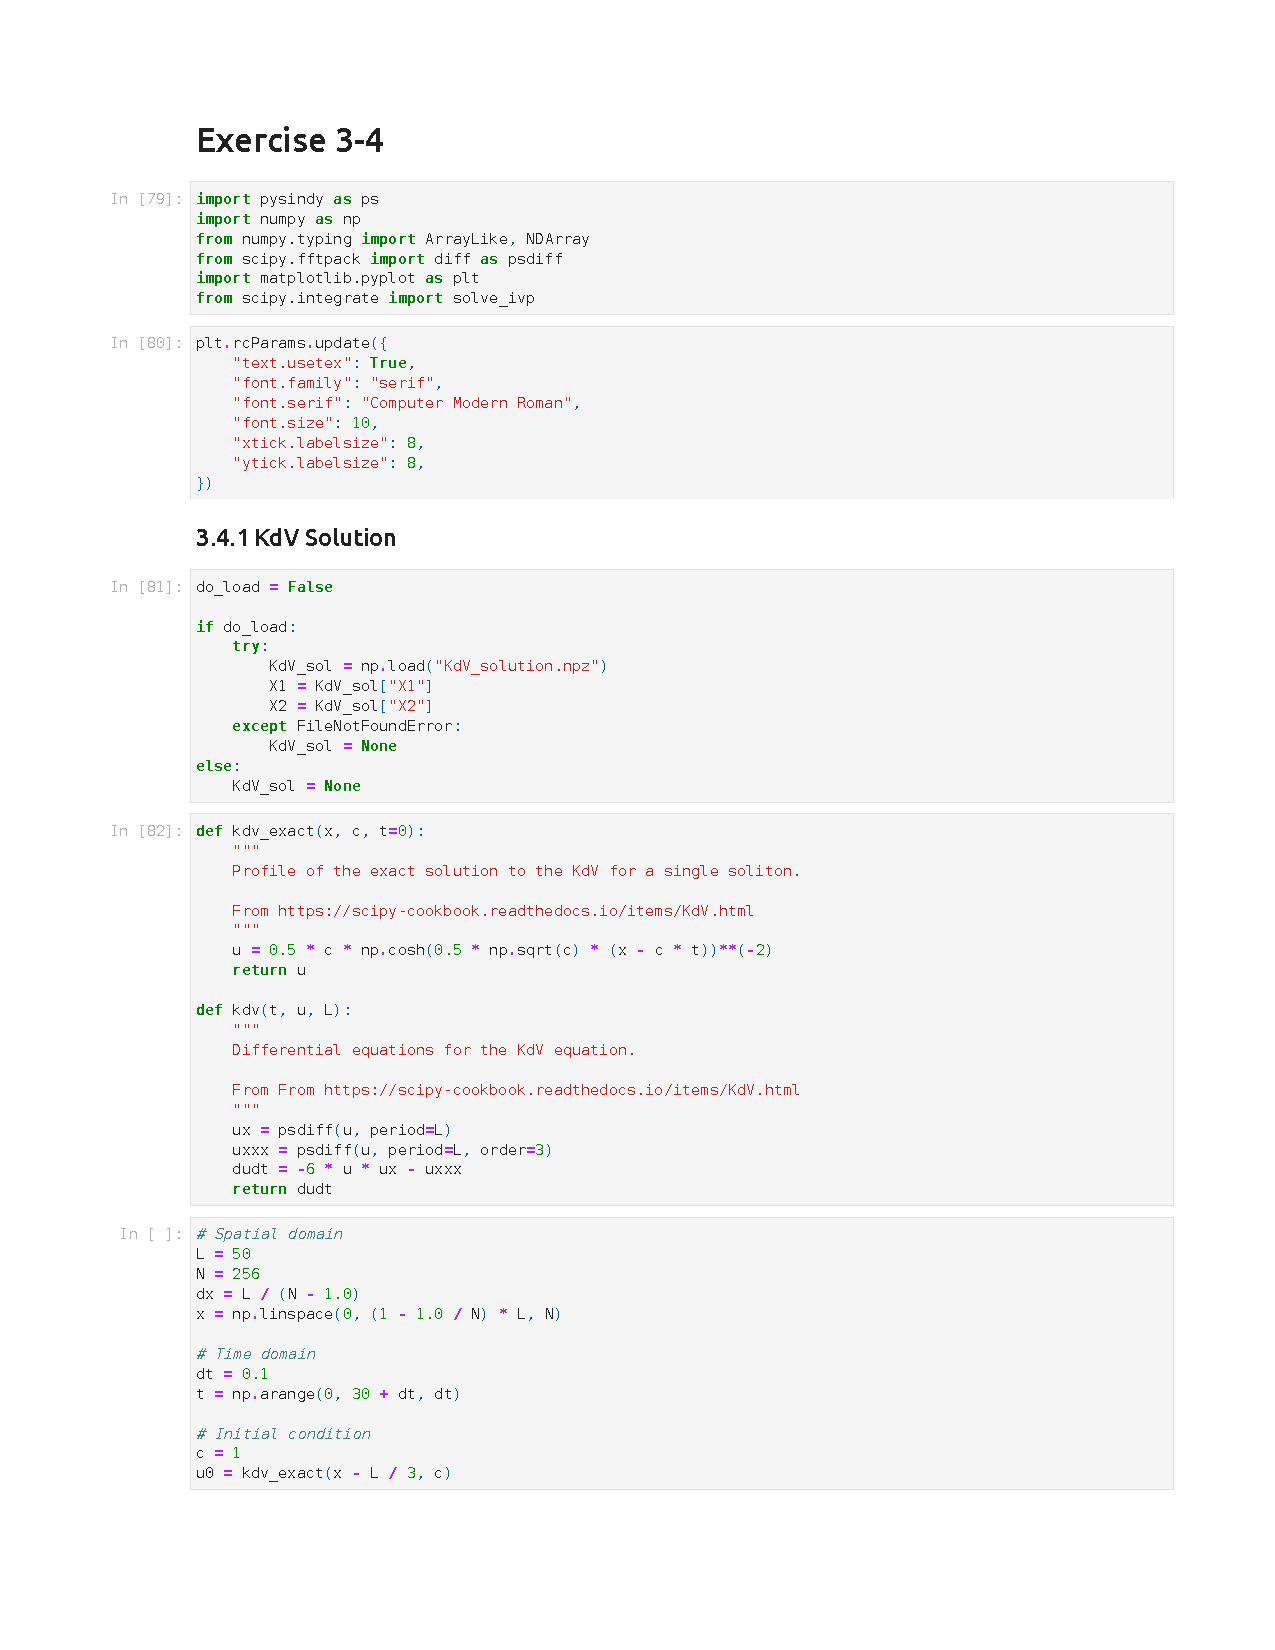
\includepdf[pages=-]{hw3p4.pdf}


\end{document}